\chapter{Self Phase Modulation}
\label{ch:SPM}

In materials with a third order nonlinearity, the refractive index at some instant depends on the optical power at that instant. Thus, a high power pulse will experience a greater change in its phase than an equivalently shaped pulse with lower power. Because many different frequencies of light can be present in a nonlinear medium at the same time, describing the impact of the nonlinearity on the optical field can be complicated. This chapter explains the simple case, labelled "Self Phase Modulation" (SPM), where only a single pulse centered at a single carrier frequency is present.  

\section{Phase change across pulse}
Starting from Eq.~\ref{eq:GNLSE} and assuming that all parameters except $\gamma>0$ are zero, that $\omega_0\A\gg\partial_T\A$ and that $R(T_{delay})=\delta(T_{delay})$, the Generalized Nonlinear Schr{\"o}dinger Equation reduces to
\begin{align}
\label{eq:SPM}
    \partial_z\A &= i\gamma|\A|^2\A.
\end{align}
Mathematically, Eq.~\ref{eq:SPM} states that for a small change in $z$, the complex number, $\A$, changes by an amount that is equal to itself rotated 90 degrees in the complex plane ($i\A$) and scaled by its own squared magnitude ($|\A|^2$) as well as a scalar, $\gamma$. Physically, Eq.~\ref{eq:SPM} implies that the nonlinearity alters the instantaneous phase of the field by an amount that depends on its power, but does not alter the magnitude of the power at that instant. Solving Eq.~\ref{eq:SPM} yields
\begin{align}
    \label{eq:SPM_applied}
    \A(z,T)&= \A(0,T)\exp\left( i\gamma|\A(0,T)|^2z \right).
\end{align}
To understand the implications of Eq.~\ref{eq:SPM_applied}, consider Eq.~\ref{eq:chirp_definition}, which states that the instantaneous frequency of a pulse is related to the negative derivative of its phase w.r.t. time.  Assuming a Gaussian pulse so that $\A(0,T)=\A_0\exp(-T^2/2T_0^2)$, the instantaneous frequency of this pulse after passing a distance, $z$, through a nonlinear medium is
\begin{align}
\label{eq:SPM_example}
    \delta\omega(z,T) &= -\gamma |\A_0|^2 z\partial_T \exp\left(-\frac{T^2}{T_0^2}\right)\\ \nonumber
    &= 2\gamma |\A_0|^2 z T/T_0^2 \exp\left(-\frac{T^2}{T_0^2}\right),
\end{align}
which implies that the pulse will develop a red-chirp in the front and a blue-chirp in the back. See Fig.~\ref{fig:chirp_profiles}(a) for a visualization of the chirp generated by a Gaussian pulse and Fig.~\ref{fig:chirp_profiles}(b-d) for visualizations of the chirps generated by other pulse profiles. Considering the argument of the exponential in Eq.~\ref{eq:SPM_applied}, a characteristic length over which nonlinear effects become significant can be defined as
\begin{align}
    L_{NL} &= \frac{1}{\gamma P_0} = \frac{1}{\gamma |\A(0,T)|^2},  
\end{align}
where $P_0$ is the initial peak power of the pulse. 

\begin{figure}
    \centering
    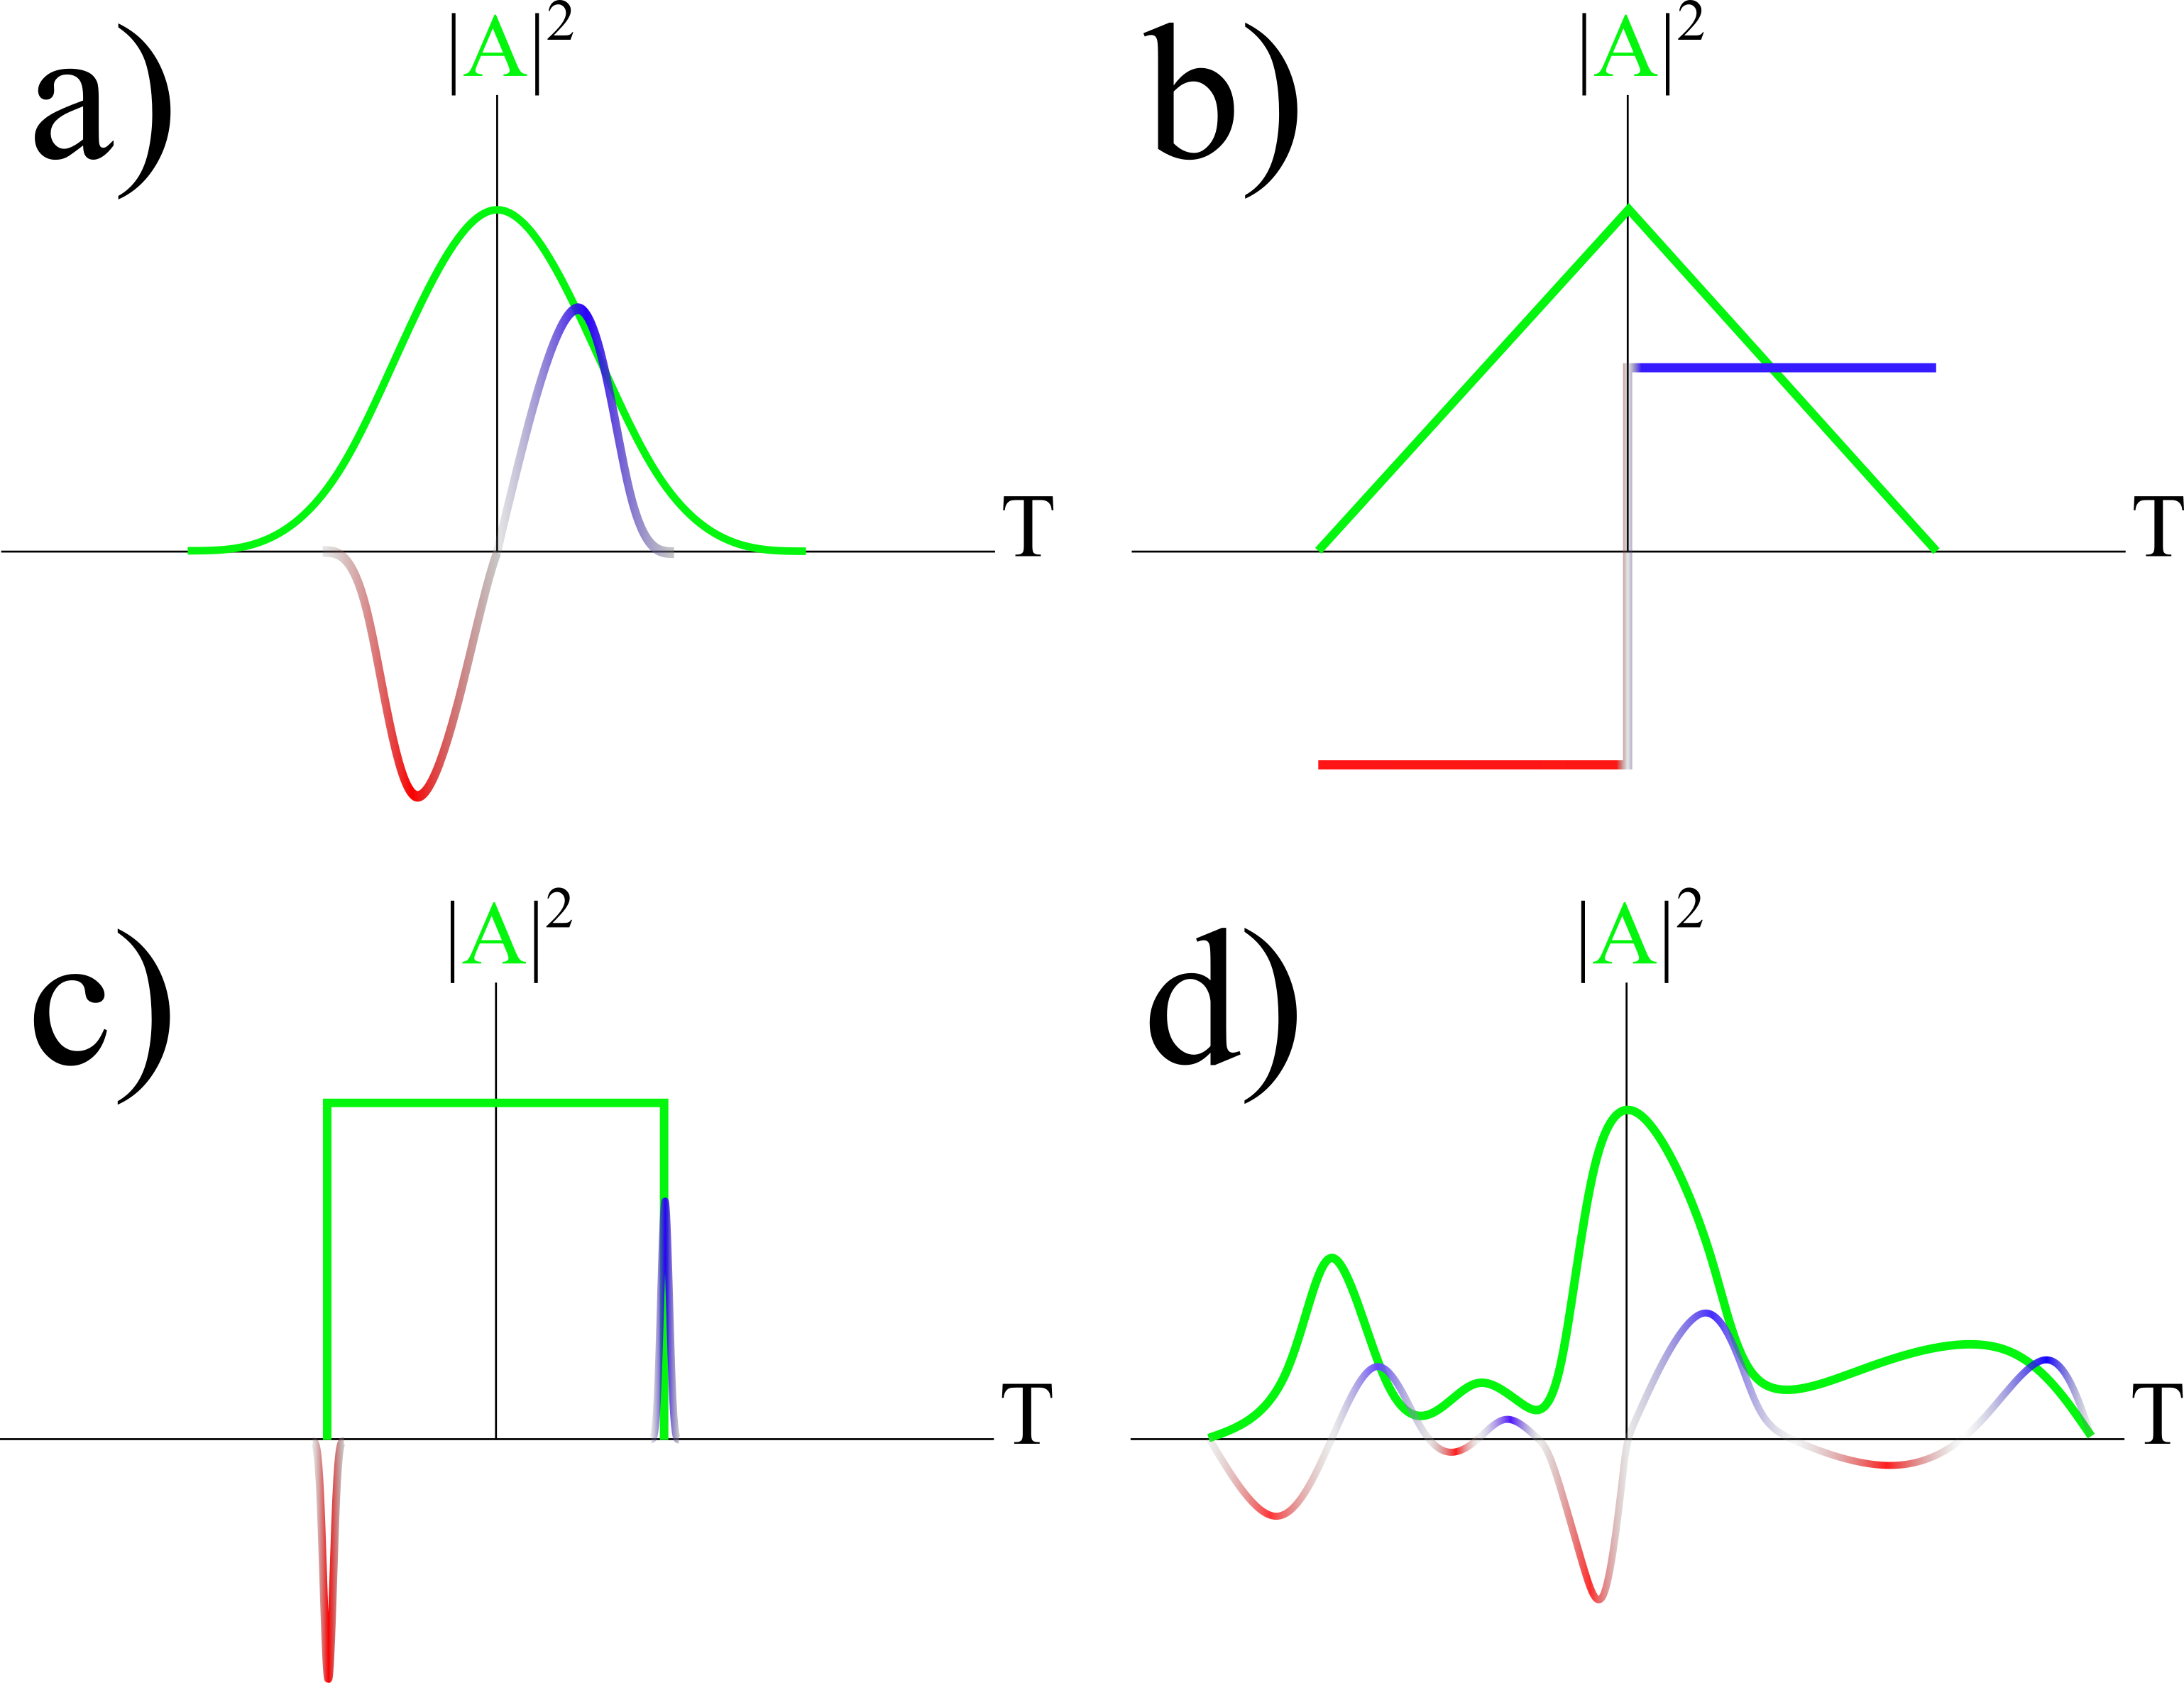
\includegraphics[width=0.75\linewidth]{figures/SPM_chirp.png}
    \caption{Visualization of the impact of SPM on a) a Gaussian pulse, b) a triangular pulse, c) a square pulse, d) an arbitrary pulse. In general, positive slopes result in a red-chirp, decreasing slope leads to a blue-chirp and horizontal slopes result in no chirp.   }
    \label{fig:chirp_profiles}
\end{figure}


\section{Spectral broadening}
The analysis of Eq.~\ref{eq:SPM_example} showed that SPM causes pulses to become "more red" at leading slopes and "more blue" at trailing slopes. Considered in isolation, $\betag_2>0$ would result in a similar behavior, but the key difference is that dispersion only changes the relative phase of different frequency components, while SPM also alters their magnitudes. In other words, SPM applied to a pulse generates new colors, which were not present initially! That Eq.~\ref{eq:SPM} implies broadening in the spectral domain can be seen mathematically by taking the Fourier Transform on both sides of the equality and recalling that the Fourier Transform of a product of two functions in the time domain is equivalent to the convolution in their spectra in the frequency domain:
\begin{align}
\label{eq:SPM_freq}
    \partial_z\Tilde{\A} &= i\gamma \FT\left\{\A\A^*\A\right\} \\ \nonumber
    &= i\gamma \Tilde{\A}*\Tilde{\A^*}*\Tilde{\A}.
\end{align}
In short, Eq.~\ref{eq:SPM_freq} implies that the change in the spectrum of $\A$ w.r.t. $z$ depends on the convolution of that spectrum with itself and its complex conjugate. Since convolving two functions yields a new function broader than the initial ones, Eq.~\ref{eq:SPM_freq} shows that the spectrum will tend to broaden with distance, implying that new frequencies are added by transferring power from the carrier towards the red and blue ends. See Fig.~\ref{fig:SPM_before_and_after} for an illustration of the impact of SPM on a Gaussian pulse.

\begin{figure}
    \centering
    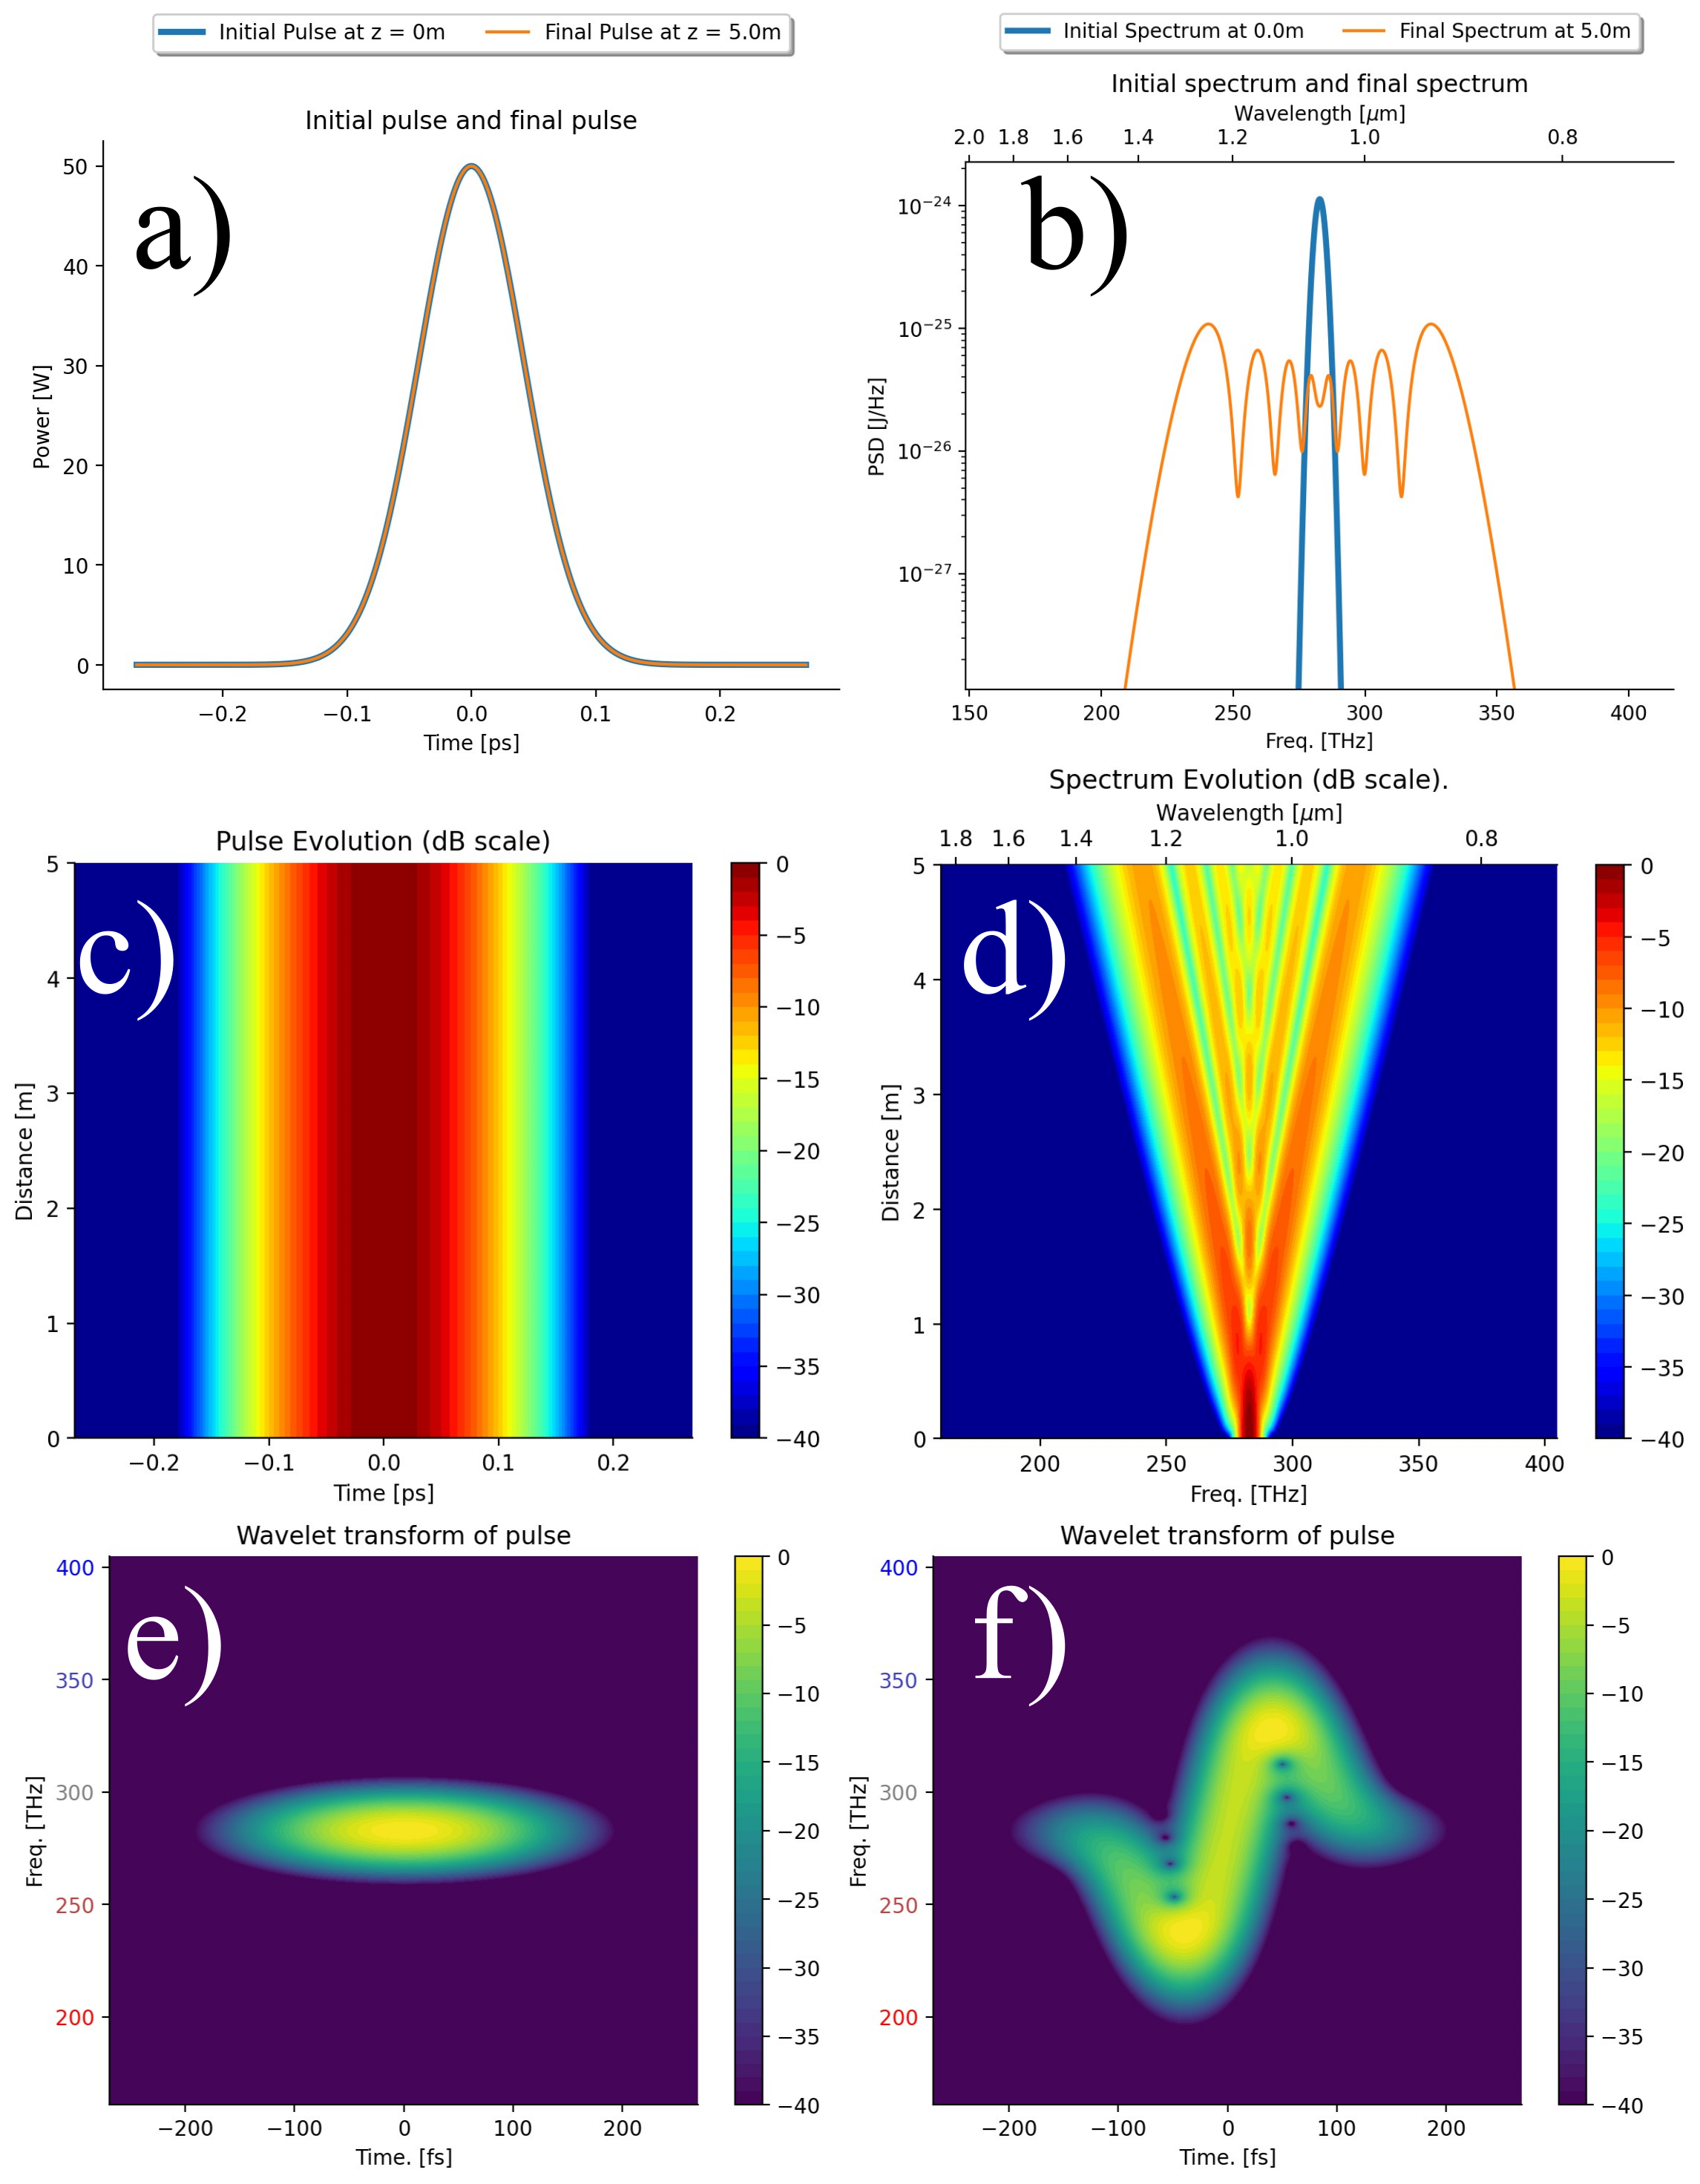
\includegraphics[width=1\linewidth]{figures/SPM_combined.png}
    \caption{ Before-and-after comparison of a Gaussian pulse propagating through a nonlinear medium described by Eq.~\ref{eq:SPM}. 
    a) In the time domain, the power envelope of the pulse is unchanged. b) The spectrum broadens. c) Evolution of the power envelope in the time domain exhibits no change. d) The spectrum gradually broadens. e) Spectrogram of pulse before propagation. f) Spectrogram of pulse after propagation. Note the broadening in the spectral domain and constant width in the temporal domain. Figures generated using the numerical simulation in \href{https://colab.research.google.com/drive/1P41F4hO6Mv12RsEkpogYv5teQyFZ6iW0?usp=sharing}{this interactive notebook}, which the reader is encouraged to experiment with.}
    \label{fig:SPM_before_and_after}
\end{figure}

 


\section{SPM, Attenuation and "Effective Length"}
Consider Eq.~\ref{eq:GNLSE} with the same assumptions as for Eq.~\ref{eq:SPM}, but where additionally $\alpha\neq0$. Recall also from Eq.~\ref{eq:attenuation_power} that $\alpha\neq0$ causes the power of the pulse to change exponentially with distance. In this case,

\begin{align}
\label{eq:SPM_and_loss}
    \partial_z\A &= \frac{\alpha}{2}\A +i\gamma|\A|^2\A\\ \nonumber
    &=\left(\frac{\alpha}{2} +i\gamma |\A(0,T)|^2 \exp(\alpha z) \right)\A. 
\end{align}
Integrating Eq.~\ref{eq:SPM_and_loss} from $0$ to $z$ yields
\begin{align}
    \label{eq:Leff_derivation}
    \A(z,T)&=\A(0,T) \exp\left( \frac{\alpha}{2}z+i\gamma|\A(0,T)|^2 \int_0^z \exp(\alpha\xi) d\xi  \right) \\ \nonumber
    &=\A(0,T) \exp\left( \frac{\alpha}{2}z+i\gamma|\A(0,T)|^2  \frac{\exp(\alpha z)-1}{\alpha}   \right) \\ \nonumber
    \A(L,T)&=\A(0,T) \exp\left( \frac{\alpha}{2}z+i\gamma|\A(0,T)|^2  L_{eff}   \right),
\end{align}
where the "Effective Length" of the medium with an actual length of $L$ is defined as
\begin{align}
\label{eq:L_eff}
    L_{eff}= \frac{\exp(\alpha L)-1}{\alpha}.
\end{align}
The insight provided by Eq.~\ref{eq:Leff_derivation} and Eq.~\ref{eq:L_eff} is that while nonlinear effects generally become more pronounced by letting the light propagate through a longer medium, the attenuation of that medium will eventually decrease the optical power to a point where all nonlinear effects become negligible. For example, the effective length of a typical 100~km single-mode fiber for telecommunications, which has a loss coefficient of $\alpha=-0.22$dB/km is approximately 19.6~km. In other words, an optical signal would accumulate approximately the same nonlinear phase shift propagating through the 100~km lossy fiber as it would have accumulated by propagating through a lossless one with a length of only 19.6km. See \href{https://www.desmos.com/calculator/g6dadbxq33}{this interactive graph} for an illustration of how the effective length depends on $\alpha$. Note that $L_{eff}\approx L$ when $\alpha L\ll 1$ and that $L_{eff}>L$ is possible when $\alpha>0$, which is the case in optical amplifiers. Furthermore, $\alpha$ may depend on $z$ in special non-uniform fibers or ones where Raman amplification is present, in which case Eq.~\ref{eq:attenuation} and thus Eq.~\ref{eq:SPM_and_loss} should be changed accordingly.   

\section{Self-Steepening}
\label{sec:SS}
In Eq.~\ref{eq:SPM}, it is assumed that the nonlinear phase shift is proportional to the field enveloped multiplied by its average power, $\A|\A|^2$. This assumption can be viewed as a zeroth-order Taylor-approximation w.r.t. time of the nonlinear response, in the same way that one can approximate $\exp(x)\approx 1$ for very small values of $x$. Assuming instead that the rate of change in the field envelope multiplied by its average power, $\partial_T(\A|\A|^2)$, also contributes yields

\begin{align}
\label{eq:SS}
    \partial_z\A &= i\gamma\left(1+\frac{i}{\omega_0}\partial_T \right)\A|\A|^2.
\end{align}
The first term in the parenthesis in Eq.~\ref{eq:SS} is SPM, while the second term is referred to as "self-steepening" (SS). Physically, this can be understood by considering that the nonlinearity causes a large change in the refractive index where the pulse power is high. A higher refractive index implies slower light propagation, causing the peak of a high power pulse to slow down relative to less intense parts as it propagates forward, thereby causing a build-up of power at later times and thus a steep, decreasing slope. Analogously, a large, unaerodynamic truck suddenly experiencing strong head-wind will slow down a lot compared to more streamlined cars and thereby cause a jam behind it, while traffic becomes less dense in front. Since SS flattens the power slope in front of the pulse and steepens it in the back, it preferentially blue-shifts the spectrum of the pulse, since $\delta\omega\propto -\partial_T|\A|^2$. See Fig.~\ref{fig:SS} for an illustration of the impact of SS on the same Gaussian pulse as in Fig.~\ref{fig:SPM_before_and_after}. For a Gaussian pulse subjected only to SPM and self-steepening, \href{https://prefetch.eu/know/concept/self-steepening/}{it can be shown} that its back slope becomes infinitely steep at a distance of
\begin{align}
    L_{SS} &= \frac{T_0\omega_0\exp(1/2)}{3\sqrt{2}\gamma P_0}.
\end{align}


See \href{https://youtu.be/Fr6yLtGZ2To}{this video tutorial} for more information on SS. 

\begin{figure}
    \centering
    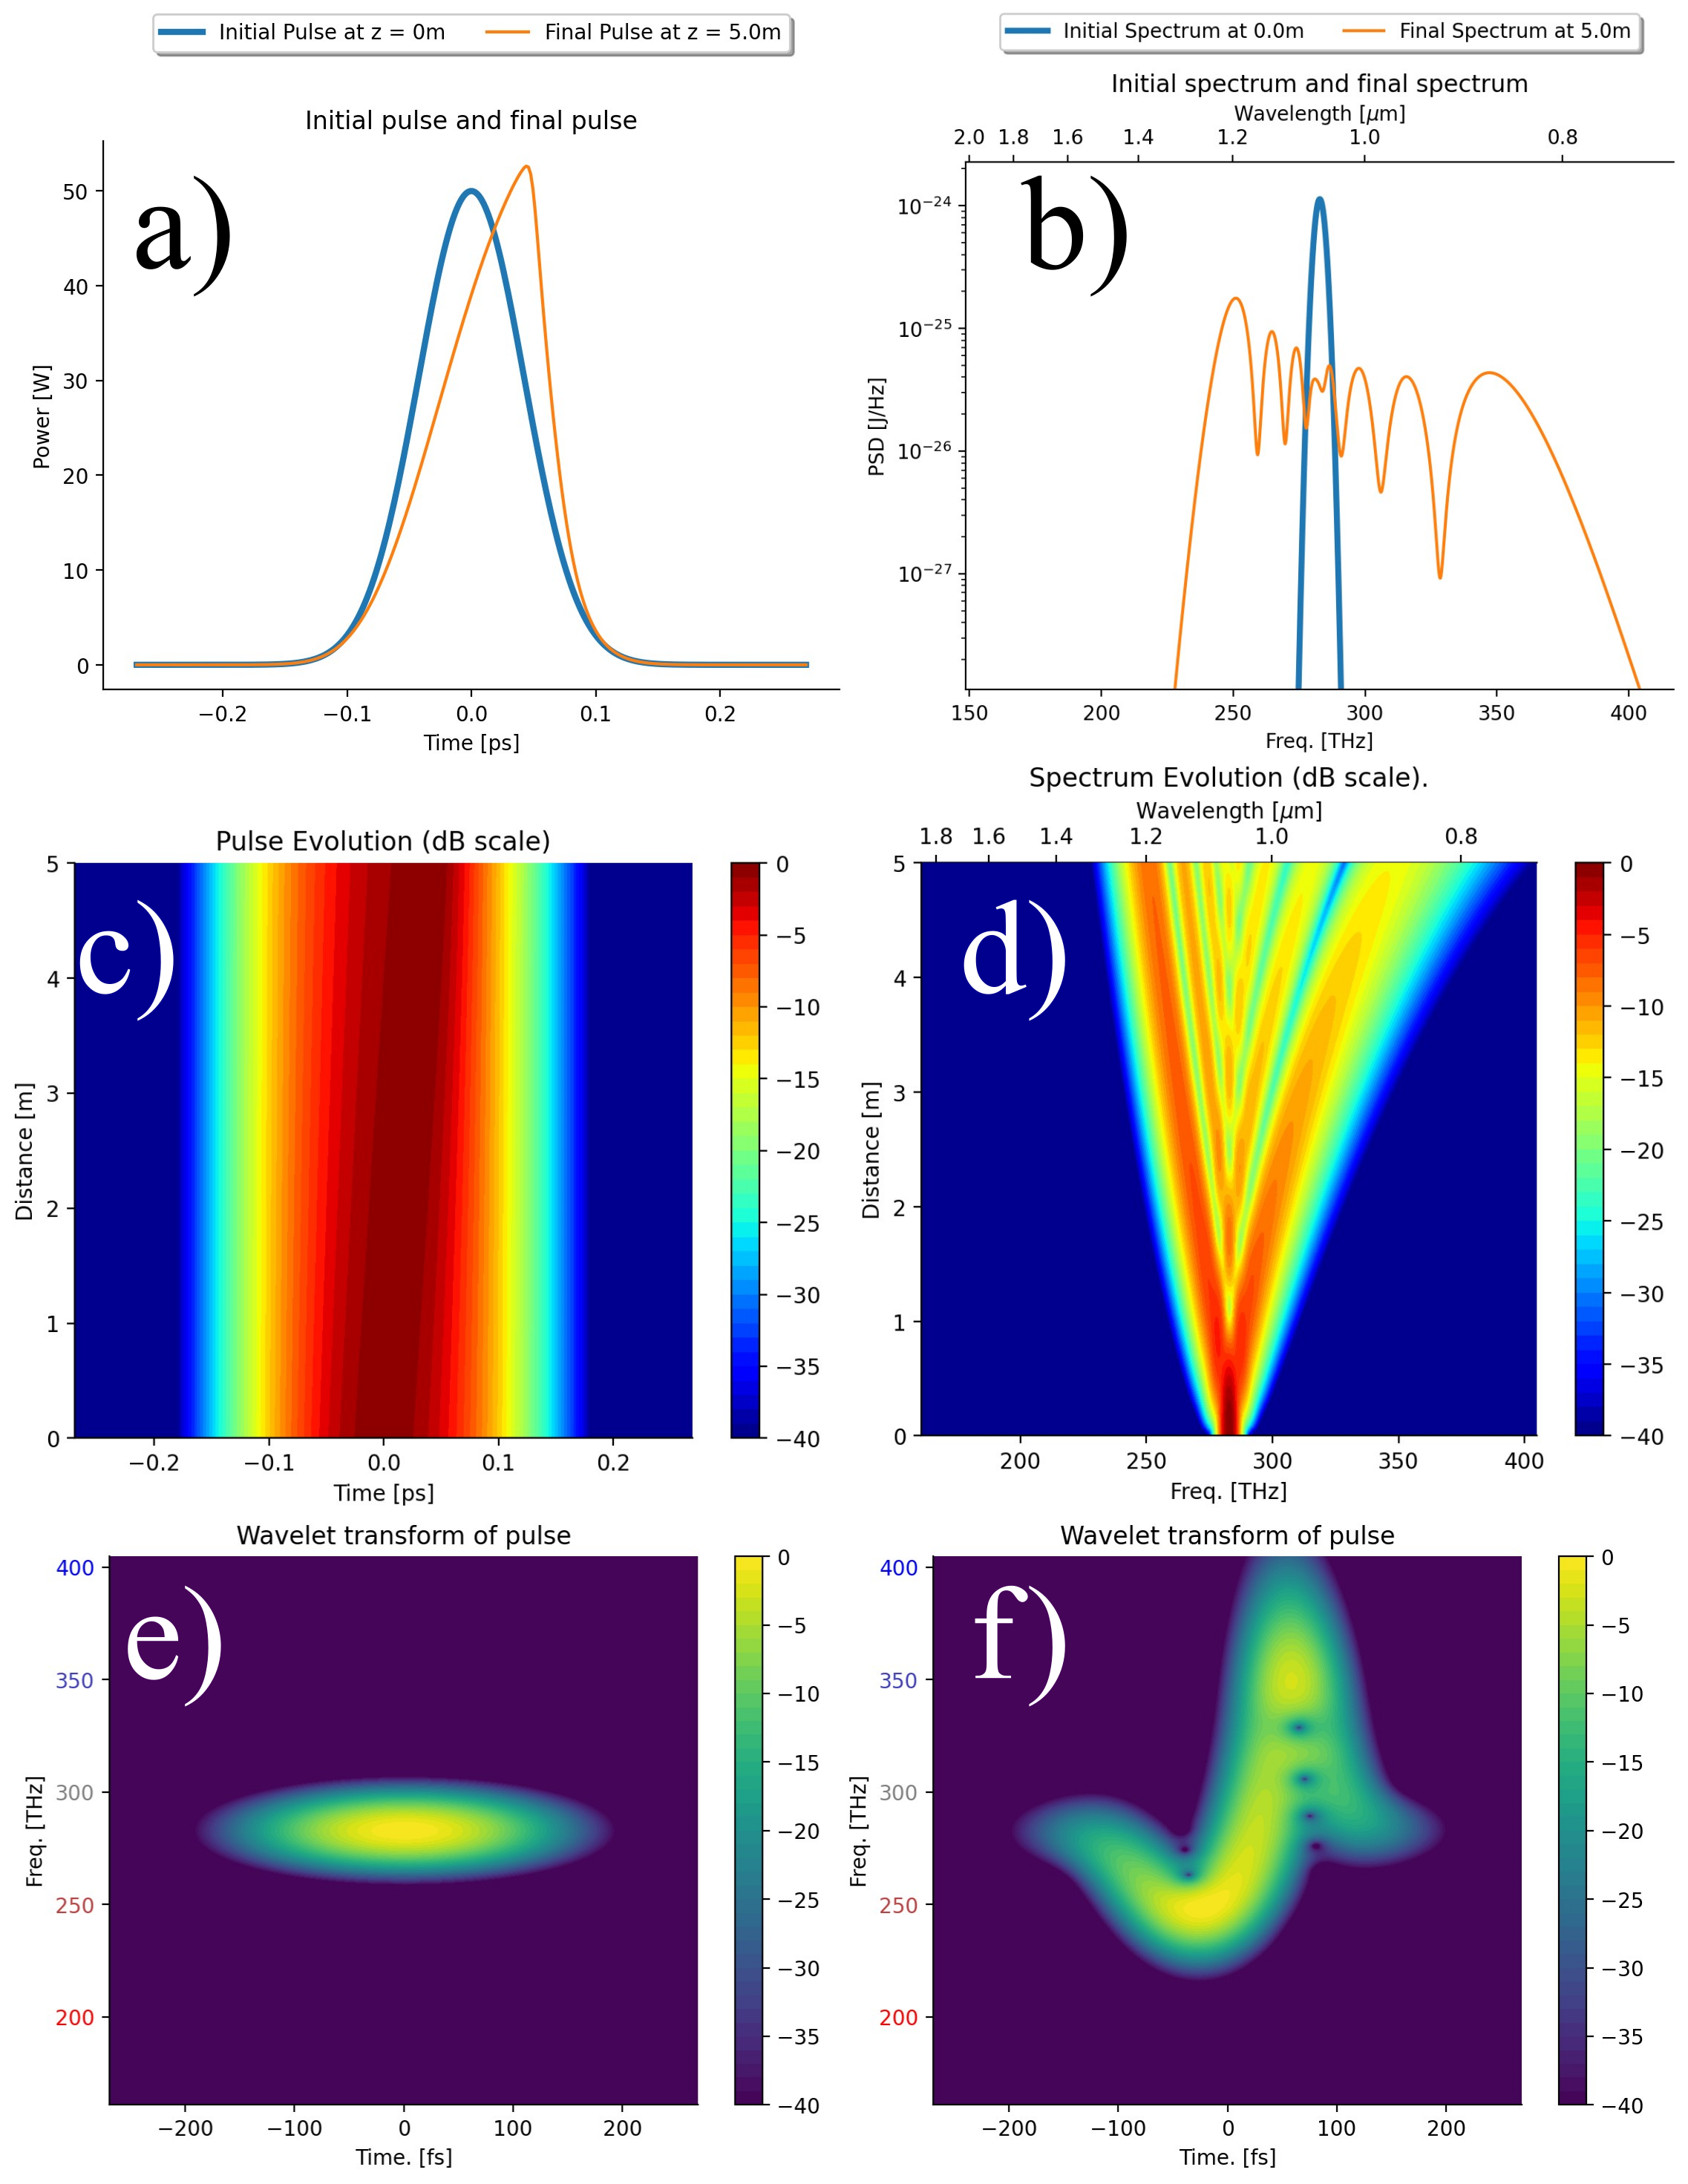
\includegraphics[width=1.0\linewidth]{figures/SPM_and_SS_combined.png}
    \caption{Before-and-after comparison of a Gaussian pulse propagating through a nonlinear medium described by Eq.~\ref{eq:SS}. 
    a) In the time domain, the power envelope of the pulse becomes steeper in the back because the peak of the pulse experiences a higher refractive index due to the nonlinearity and slows down. b) The spectrum broadens asymetrically towards higher frequencies due to the steep, decreasing slope in the back. c) Evolution of the power envelope in the time domain. d) The spectrum gradually broadens towards higher frequencies. e) Spectrogram of pulse before propagation. f) Spectrogram of pulse after propagation. Figures generated using the numerical simulation in \href{https://colab.research.google.com/drive/1P41F4hO6Mv12RsEkpogYv5teQyFZ6iW0?usp=sharing}{this interactive notebook}, which the reader is encouraged to experiment with. }
    \label{fig:SS}
\end{figure}

\subsection{Applicability}
Since the impact of SS is inversely proportional to $\omega_0\approx 2\pi/200~\text{THz} = 2\pi/5$fs and the time derivative of $\A|\A|^2$ is small for long pulses, SS is significant for pulse durations below 100~fs, somewhat significant for pulse durations on the scale of 100s of fs and negligible for pulse durations longer than a few ps. 




